\section{Results}
\label{sec:Results}

The results of an SVM on the data sets is presented in Section \ref{sec:Results_ParamSearch}.
In Section \ref{sec:Results_AdaBoost} the results are shown for using an ensamble methods.

\subsection{Parmater Search}
\label{sec:Results_ParamSearch}

The parameter search for the optimal C and $\sigma$ parameters is shown in the contour plots of Figures \ref{fig:ParamLiver}, \ref{fig:ParamGlass} and \ref{fig:ParamGlass}.
The optimal classifier parameters are shown for the coarse parameter search in Table \ref{tab:CoarseParamValues} and for the fine parameter search in Table \ref{tab:FineParamValues}.
\todo{Make some quantifications and discuss the data}
\begin{table}[h!]
\caption{Coarse Optimal Classifier Parameters}
\label{tab:CoarseParamValues}
\centering
\begin{tabular}{c c c c c c c c}
\hline
\input{../CoarseGridSearchOutput.dat}
\hline
\end{tabular}
\end{table}
\begin{table}[!ht]
\caption{Fine Optimal Classifier Parameters}
\label{tab:FineParamValues}
\centering
\begin{tabular}{c c c c c c c c}
\hline
\input{../FineGridSearchOutput.dat}
\hline
\end{tabular}
\end{table}
\begin{figure*}[!ht]
	\centering
	\begin{subfigure}[b]{0.4\textwidth}
		\centering
		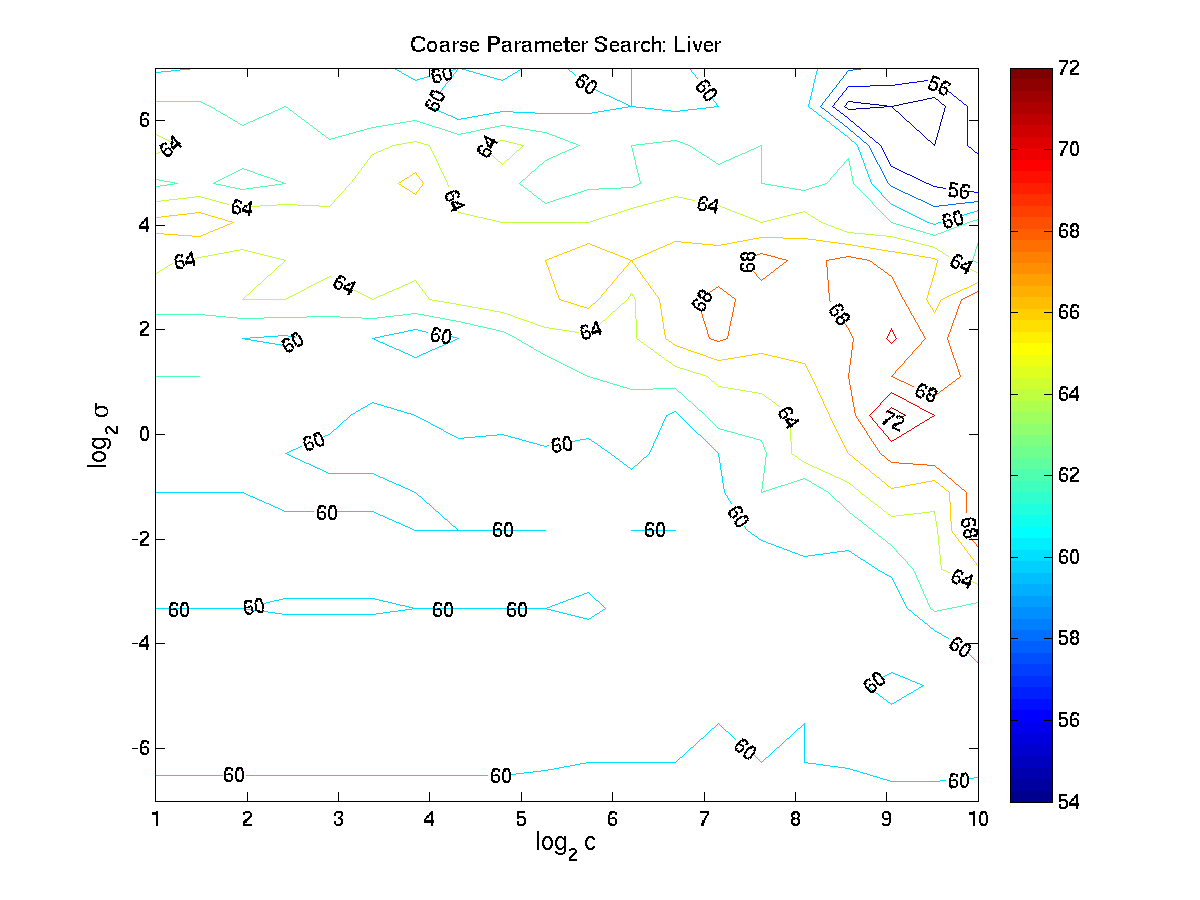
\includegraphics[width=\textwidth]{Liver_coarseSearch}
        \caption{Coarse Search}
	\end{subfigure}%
	~
	\begin{subfigure}[b]{0.4\textwidth}
		\centering
		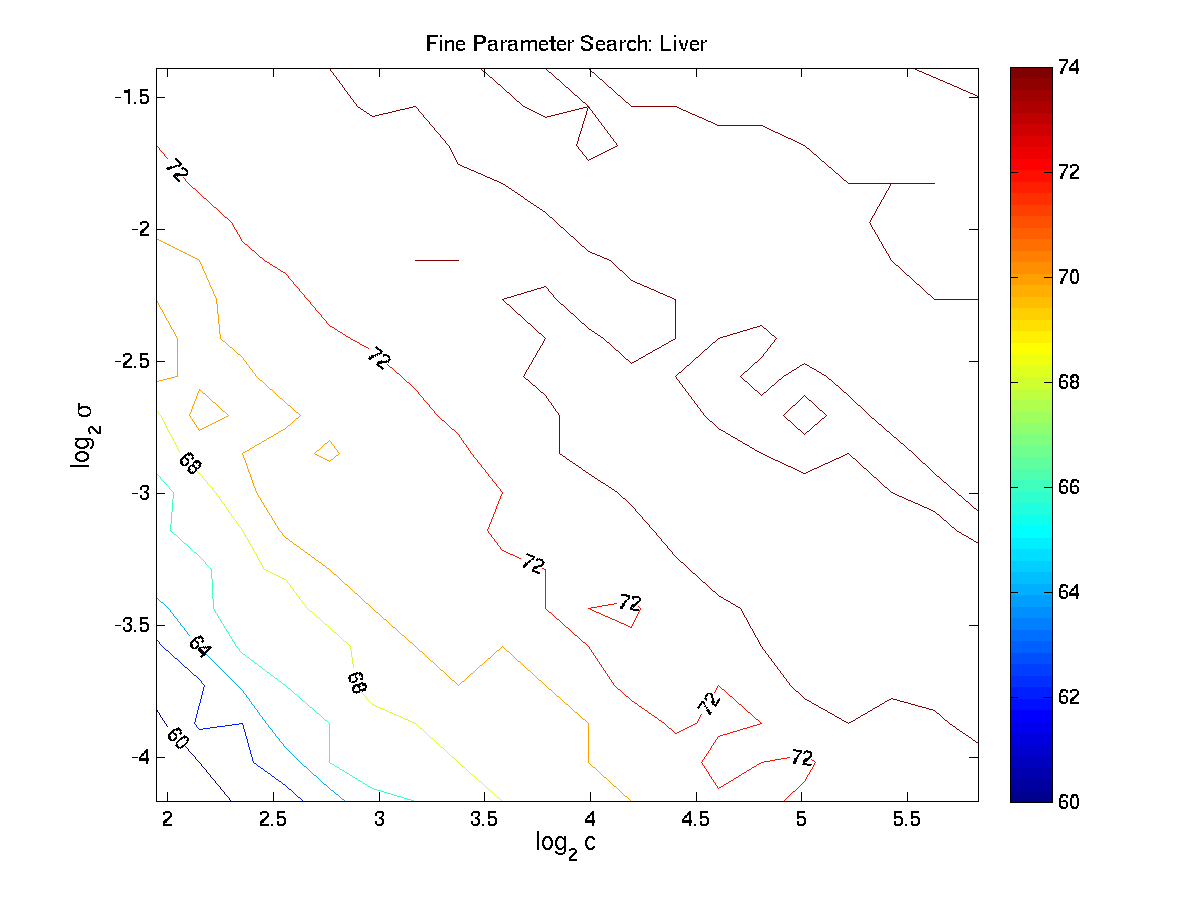
\includegraphics[width=\textwidth]{Liver_fineSearch}
        \caption{Fine Search}
	\end{subfigure}	
	\caption{Parameter search for Liver Disorder}
	\label{fig:ParamLiver}

	\begin{subfigure}[b]{0.4\textwidth}
		\centering
		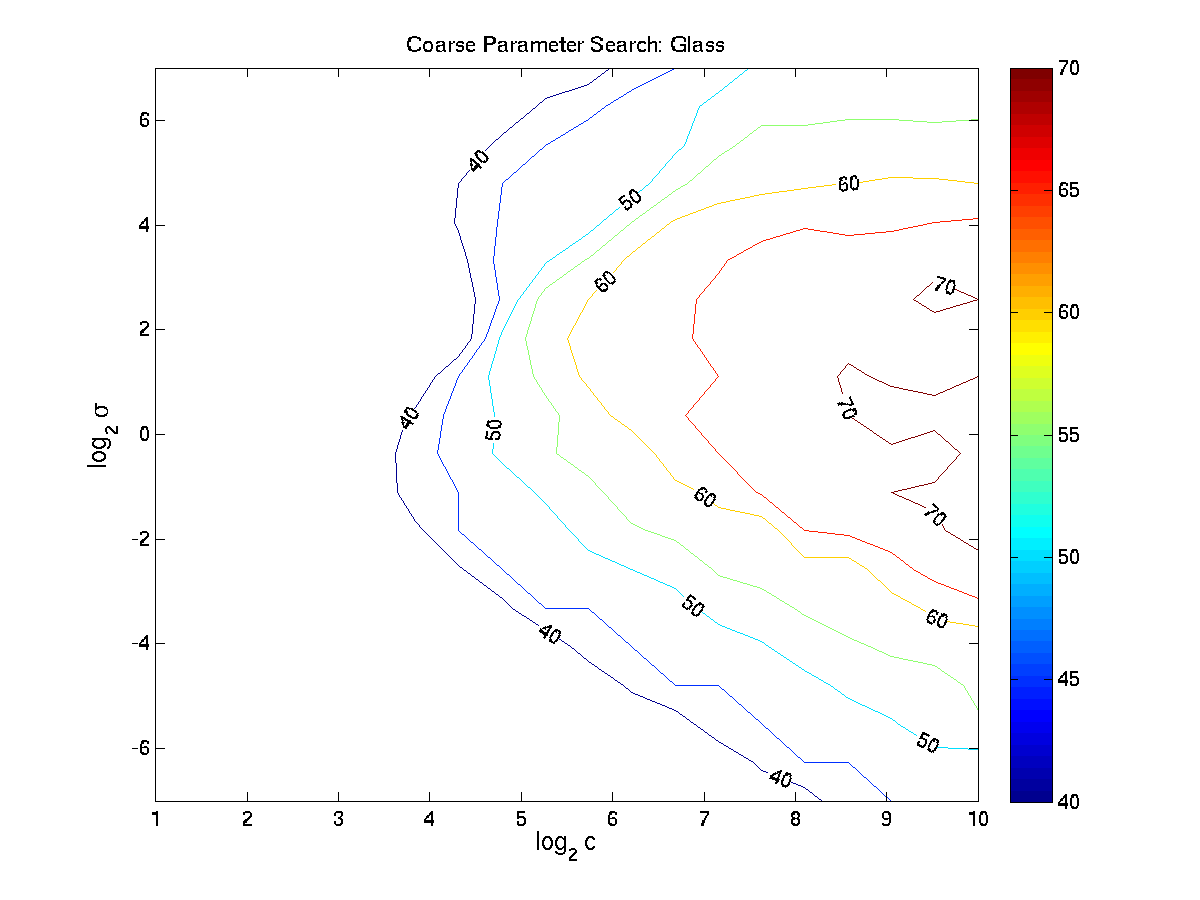
\includegraphics[width=\textwidth]{Glass_coarseSearch}
        \caption{Coarse Search}
	\end{subfigure}%
	~
	\begin{subfigure}[b]{0.4\textwidth}
		\centering
		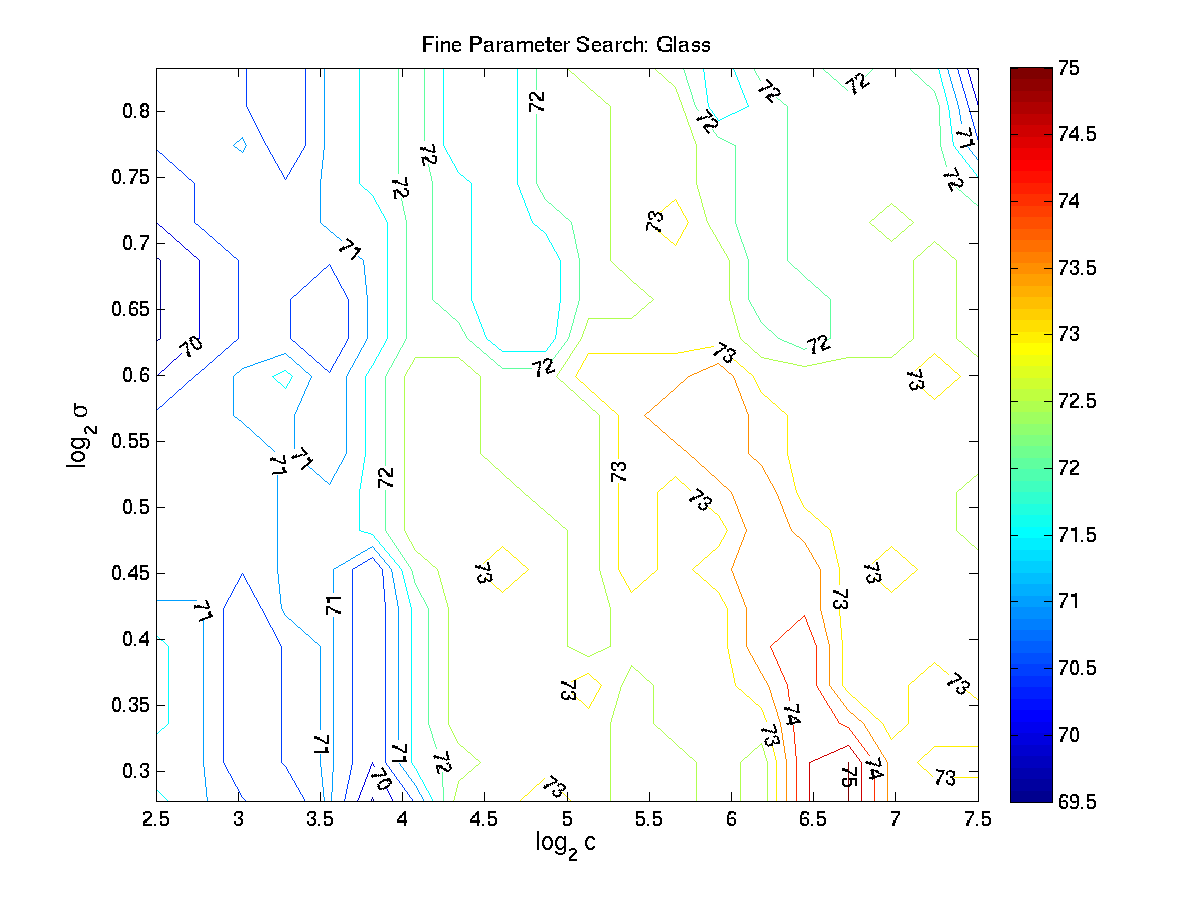
\includegraphics[width=\textwidth]{Glass_fineSearch}
        \caption{Fine Search}
	\end{subfigure}	
	\caption{Parameter search for Glass Disorder}
	\label{fig:ParamGlass}

	\begin{subfigure}[b]{0.4\textwidth}
		\centering
		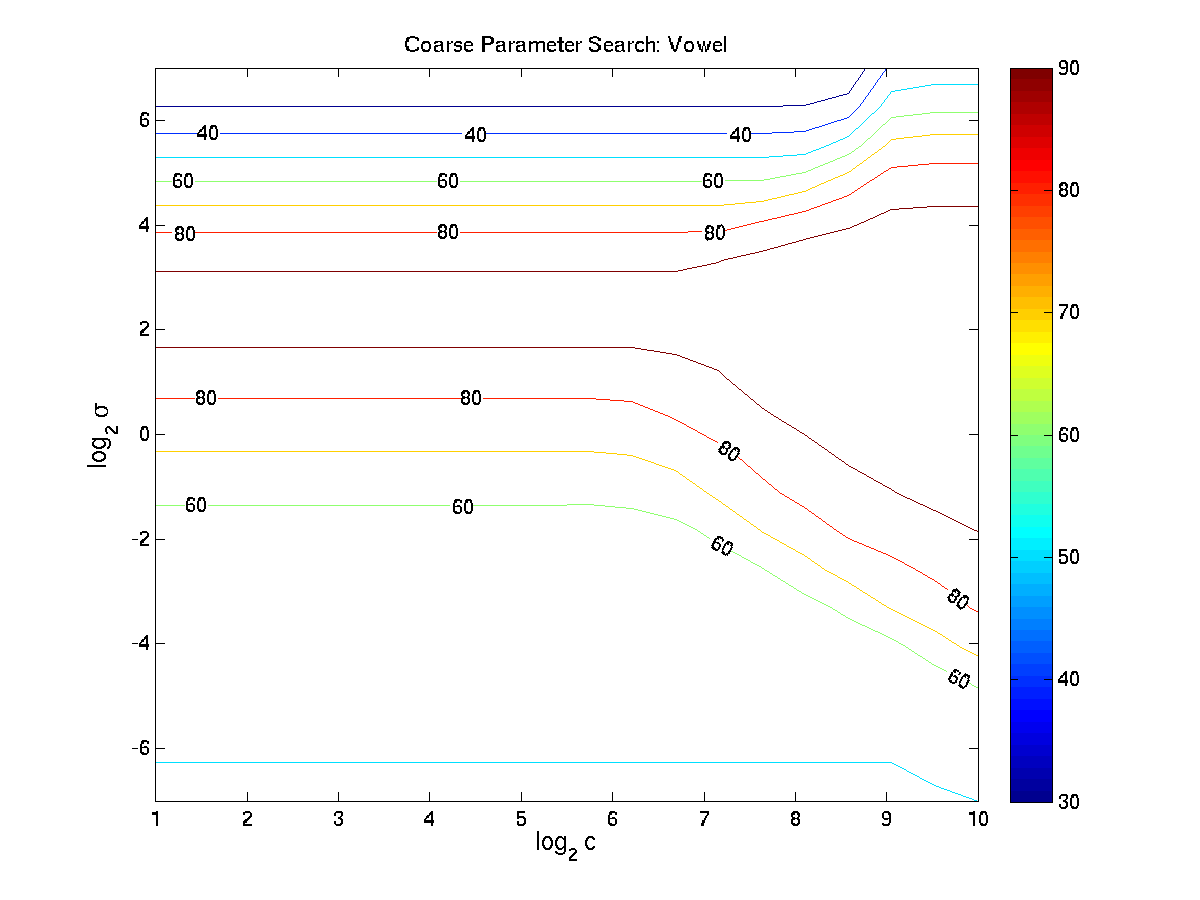
\includegraphics[width=\textwidth]{Vowel_coarseSearch}
        \caption{Coarse Search}
	\end{subfigure}%
	~
	\begin{subfigure}[b]{0.4\textwidth}
		\centering
		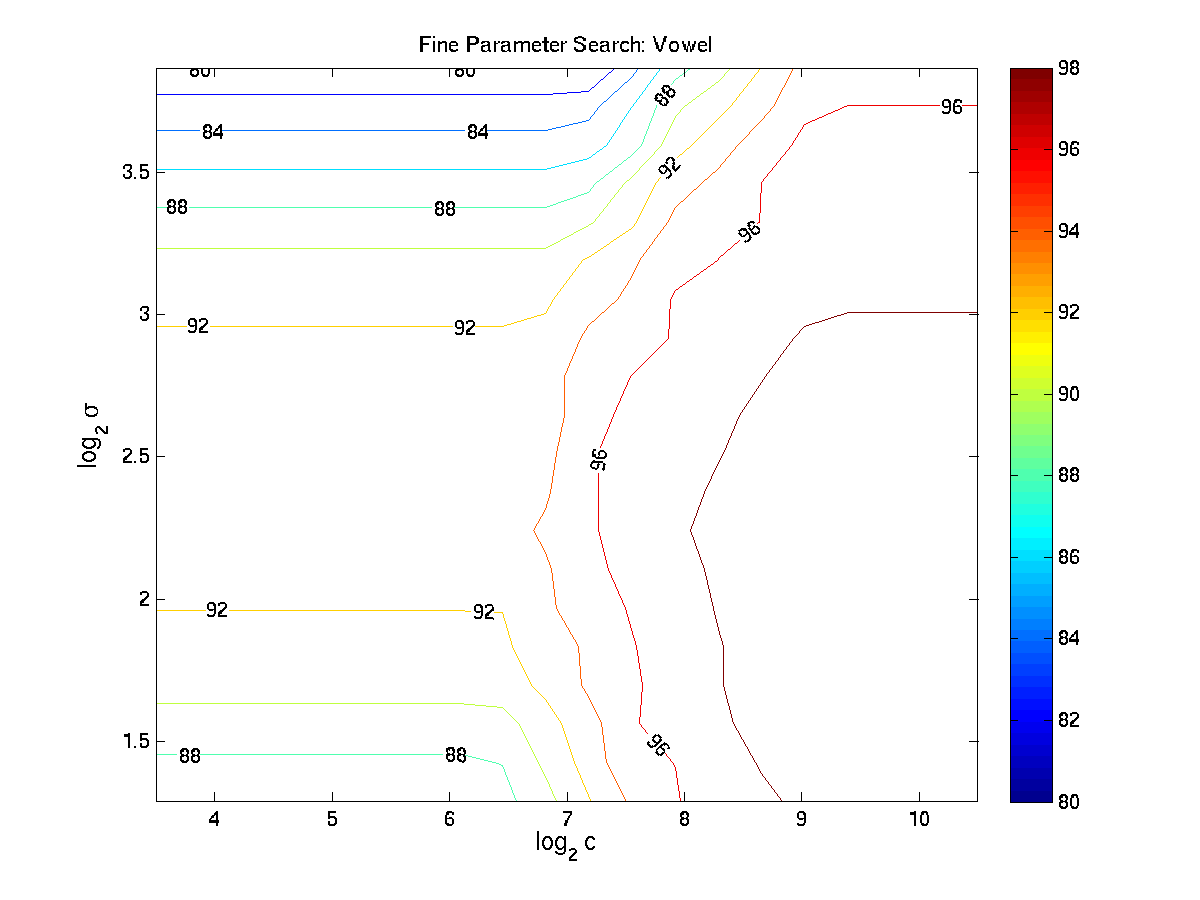
\includegraphics[width=\textwidth]{Vowel_fineSearch}
        \caption{Fine Search}
	\end{subfigure}	
	\caption{Parameter search for Vowel Disorder}
	\label{fig:ParamVowel}
\end{figure*}

\subsection{AdaBoostM1}
\label{sec:Results_AdaBoost}
The results using the implemented AdaBoostM1 algorthim are shown below in Table \ref{tab:AdaBoostValues}.
It is immediately observablve that the AdaBoost algorthim increased the accuarcy of the the Liver and Glass data set, but failed to increase (in fact dramatically lowered) the accuaracy for the Vowel data set.
\begin{table}[!ht]
\caption{AdaBoost Classifer Values}
\label{tab:AdaBoostValues}
\centering
\begin{tabular}{c c c c c}
\hline
\input{../AdaBoostOutput_50.dat}
\\
\hline
\input{../AdaBoostOutput_100.dat}
\hline
\end{tabular}
\end{table}

The effect of the number of the classifers in the ensamble is shown in Figure \ref{fig:AccuracyEnsambleSize}.
\begin{figure}[!ht]
    \centering
    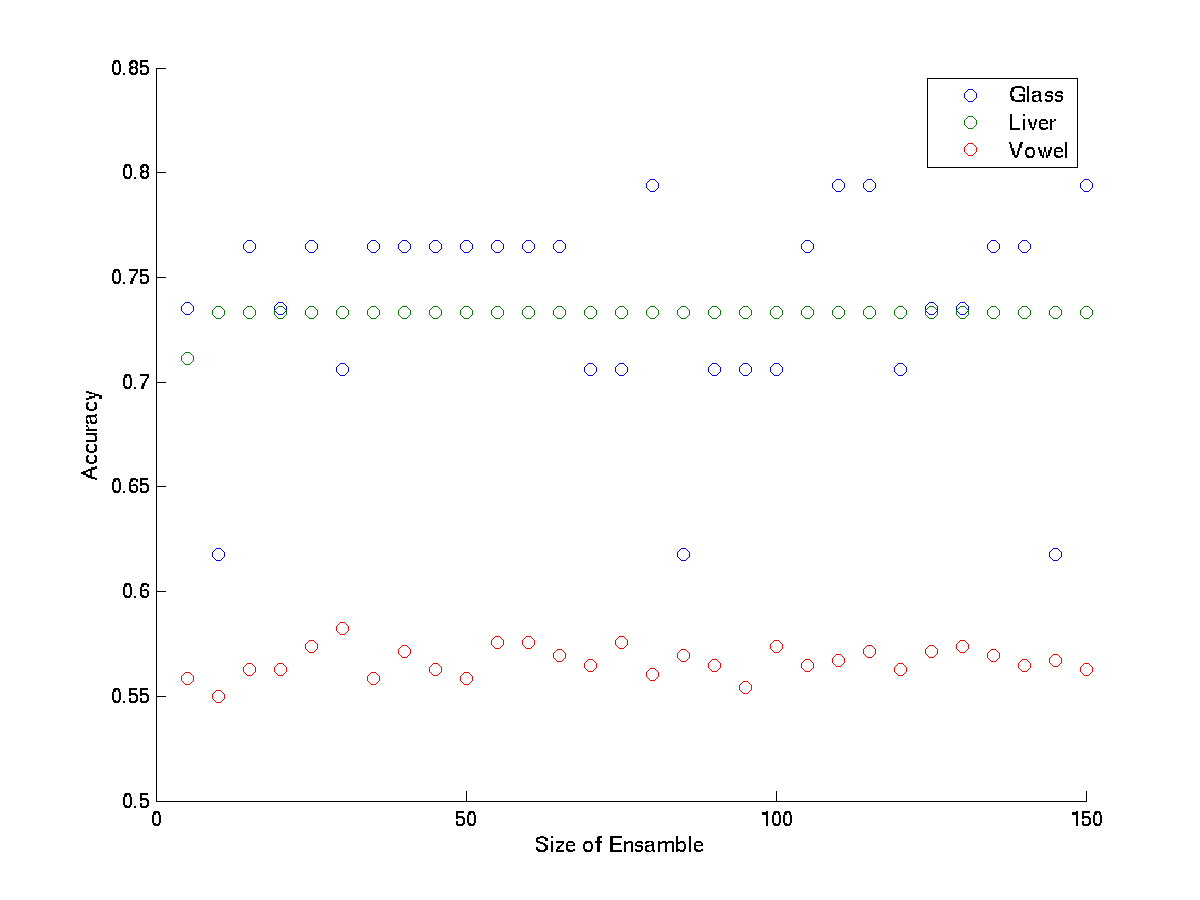
\includegraphics[width=0.45\textwidth]{AccuracyVSEnsambleSize}
    \caption{Accuracy and Number of Compenents in Ensamble}
    \label{fig:AccuracyEnsambleSize}
\end{figure}
The weight of each individual classifer for an ensamble of 150 members is shown in Figure \ref{fig:EnsambleWeights}
\begin{figure*}[ht!]
	\centering
	\begin{subfigure}[b]{0.3\textwidth}
		\centering
		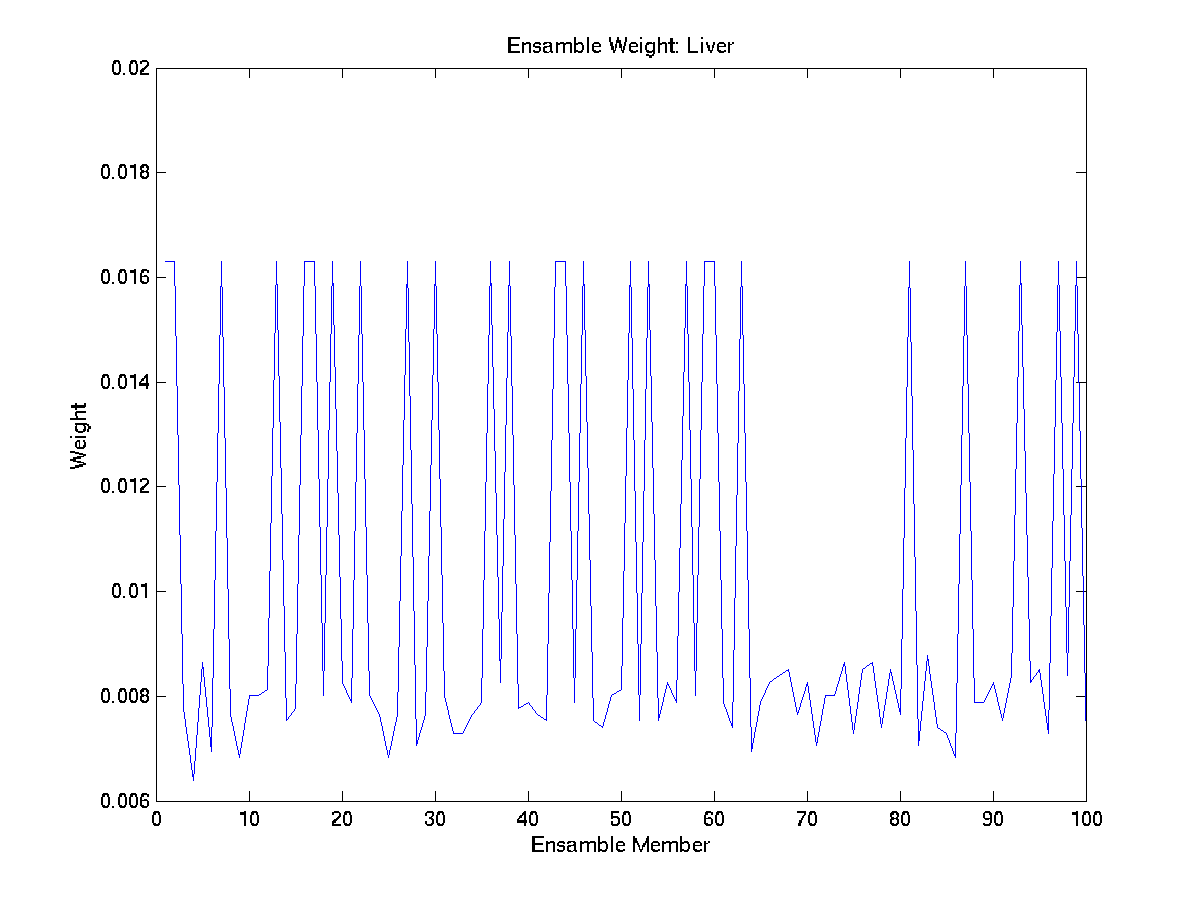
\includegraphics[width=\textwidth]{Liver_EnsambleWeight}
      \caption{Liver}
	\end{subfigure}%
	~
	\begin{subfigure}[b]{0.3\textwidth}
		\centering
		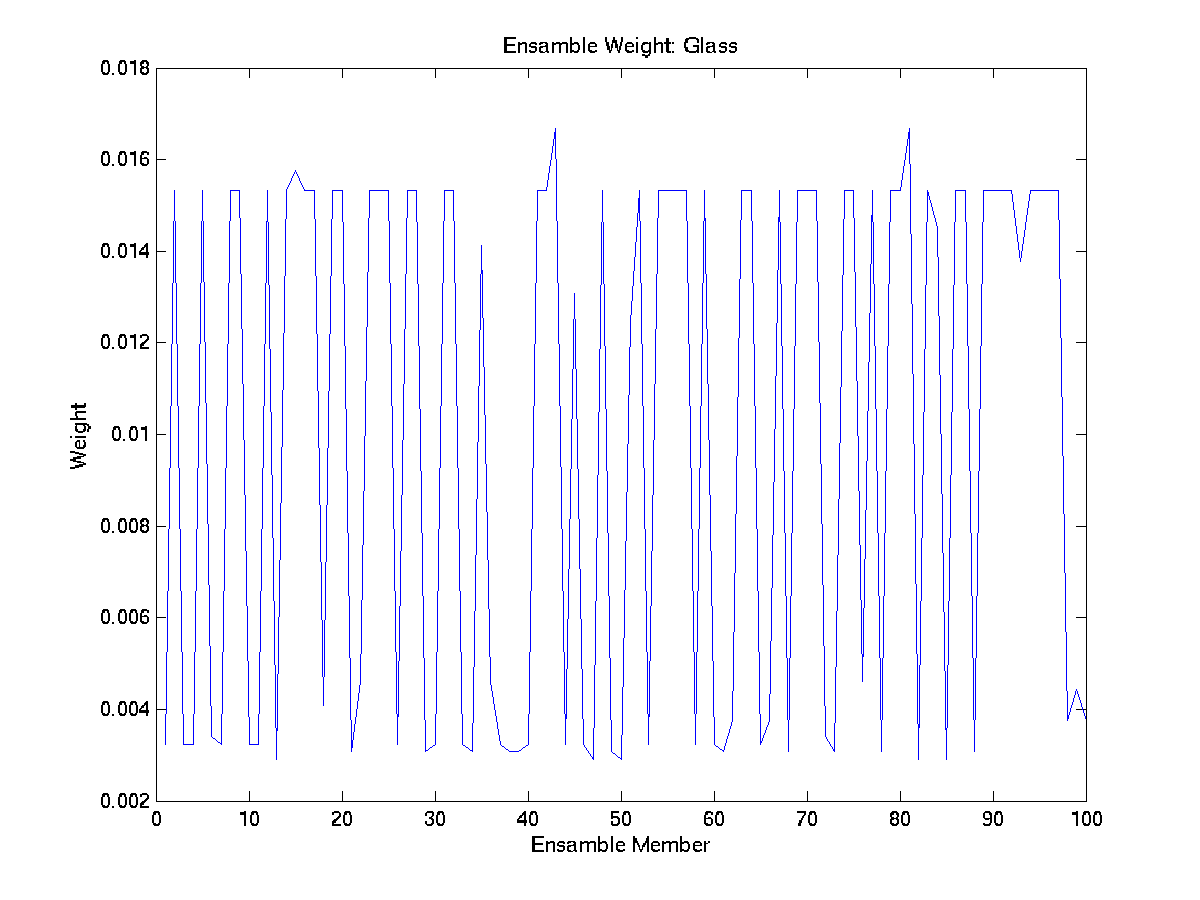
\includegraphics[width=\textwidth]{Glass_EnsambleWeight}
        \caption{Glass}
	\end{subfigure}	
    ~
	\begin{subfigure}[b]{0.3\textwidth}
		\centering
		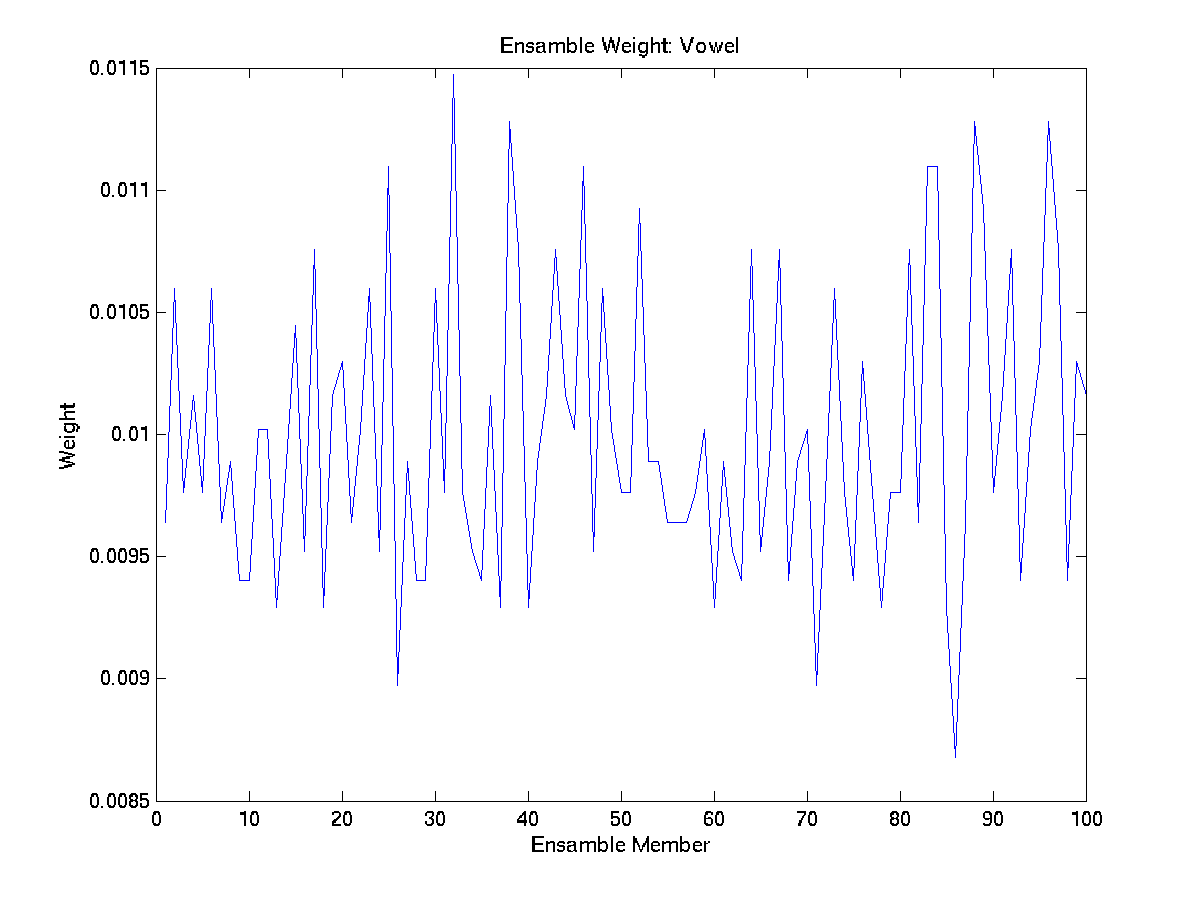
\includegraphics[width=\textwidth]{Vowel_EnsambleWeight}
        \caption{Vowel}
	\end{subfigure}%
	\caption{Distribution of Ensamble Weights}
	\label{fig:EnsambleWeights}
\end{figure*}
